%%% template.tex
%%%
%%% This LaTeX source document can be used as the basis for your technical
%%% paper or abstract. Intentionally stripped of annotation, the parameters
%%% and commands should be adjusted for your particular paper - title, 
%%% author, article DOI, etc.
%%% The accompanying ``template.annotated.tex'' provides copious annotation
%%% for the commands and parameters found in the source document. (The code
%%% is identical in ``template.tex'' and ``template.annotated.tex.'')

\documentclass[annual]{acmsiggraph}

\usepackage{array}
\usepackage[justification=centering]{caption}
\usepackage{subfigure}

\TOGonlineid{}
\TOGvolume{0}
\TOGnumber{0}
\TOGarticleDOI{}
\TOGprojectURL{http://GPUTerrain.blogspot.com/}
\TOGvideoURL{}
\TOGdataURL{}
\TOGcodeURL{https:://github.com/tijutv/GPU-Terrain-Generation}

\title{Terrain Generation on the GPU using Tessellation Shaders}

\author{Tiju Thomas V.\thanks{e-mail:tijutv@gmail.com}\\University of Pennsylvania}
\pdfauthor{Tiju Thomas V.}

\keywords{terrain, tessellation shaders, procedural, heightmap, OpenGL}

\begin{document}

 \teaser{
 \subfigure[Tessellated Mesh]{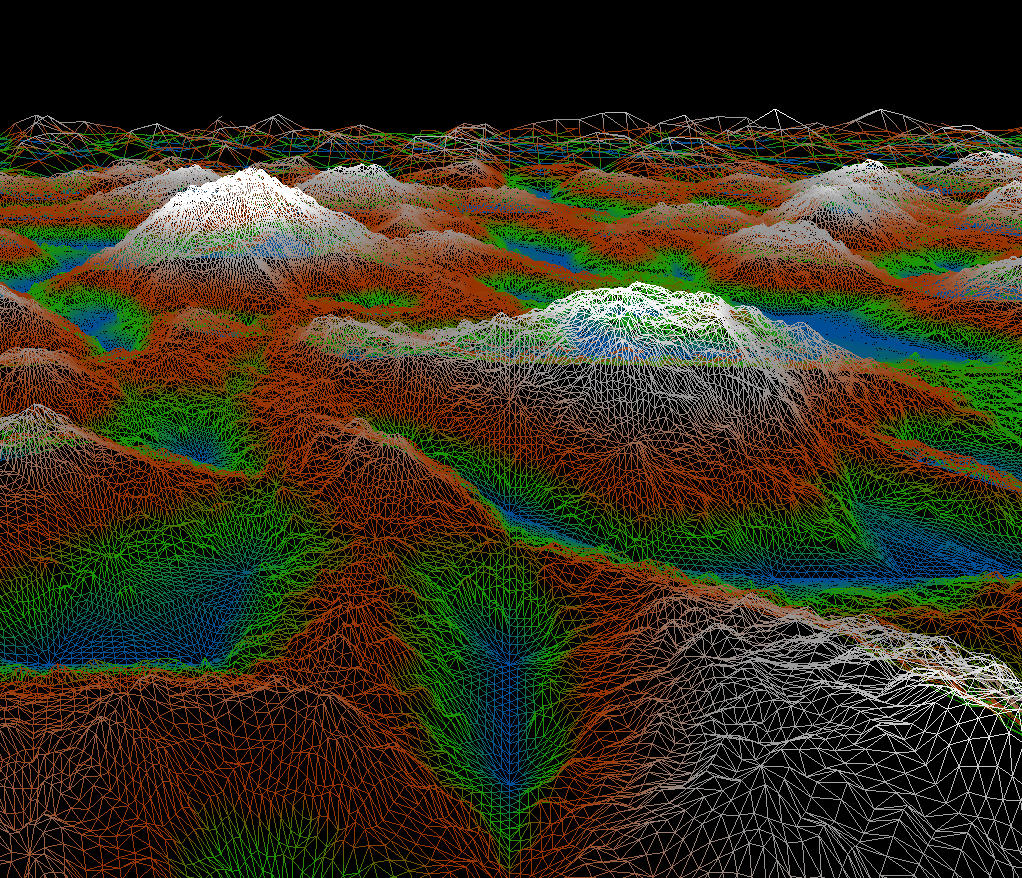
\includegraphics[height=2.8in]{images/TessMesh.png} \label{fig:meshTess}}
 \hspace{0.2in}
    \subfigure[Tessellated and Shaded Terrain with fog, based on depth and height]{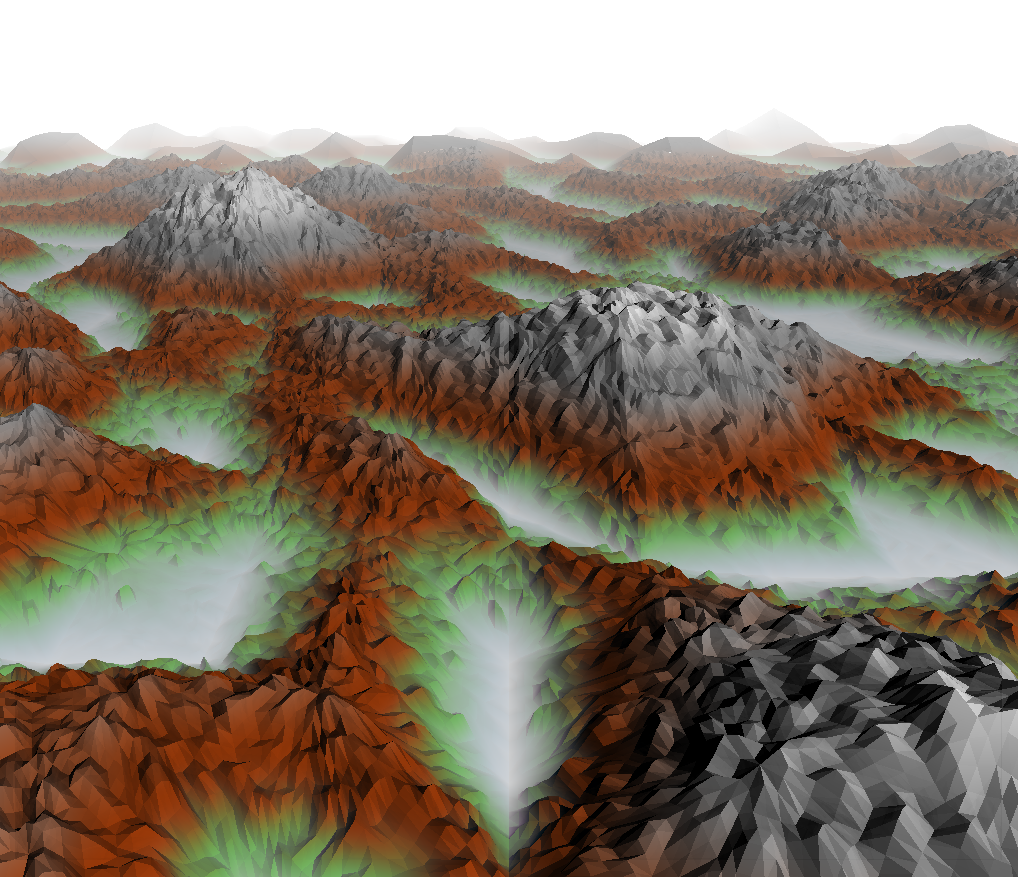
\includegraphics[height=2.8in]{images/TessMeshShaded.png}  \label{fig:meshShaded}}
    \hspace{0.2in}
    \caption{Terrain generated based on Perlin noise and tessellated based on distance from the camera}
\label{fig:mesh}
}

\maketitle

\begin{abstract}

Terrain Generation is extensively used in games and movies. But one of the challenges faced is that it takes a long time to create a terrain on the CPU.  Highly detailed terrains have a negative impact on  performance. The technique used for generating terrains work on vertices independently, which enables us to parallelize the algorithm and implement it on the GPU. In this paper, I propose a method of generating terrain on the GPU making use of the tessellation shaders present in the modern OpenGL pipeline. The tessellation shaders can be used based on distance of the terrain from the camera, thus giving a highly detailed surface close to the camera, with the details decreasing as we look into the distance.

\end{abstract}

%%\begin{CRcatlist}
%%  \CRcat{I.3.3}{Computer Graphics}{Three-Dimensional Graphics and Realism}{Display Algorithms}
%%  \CRcat{I.3.7}{Computer Graphics}{Three-Dimensional Graphics and Realism}{Radiosity};
%%\end{CRcatlist}

\keywordlist

\TOGlinkslist

\copyrightspace

\section{Introduction}

Terrain generation is used to create landscapes and forests based on random values or from data obtained through elevation maps. If the algorithm is executed on the CPU, it has an effect on the performance and doesn't make use of the parallelism which is inherently present in the generation technique. Detailed terrains have millions of vertices which can be executed in parallel on the GPU.

In this paper, the first section provides an overview of the different shaders used for terrain generation. The next section gives details of the render passes. The other sections cover functionalities added to the terrain for visual enhancements. The performance of the present algorithm and future steps to improve the final output have also been discussed.

\section{Related Work}
A number of articles discuss the different techniques used for terrain generation. ~\cite{Ebert:2003} describes how to generate terrain using Perlin noise. It also describes Perlin noise in detail. The book also covers on how to generate variety of terrains using different noise functions. ~\cite{GPUGems3:2007} uses a voxel based method along with noise to generate the terrain. None of the above references have used the new Tessellation shader available since OpenGL 4.0.

~\cite{openglInsights:2012} and ~\cite{grasshopper:2010} describe how tessellation works in the OpenGL pipeline and how it can be used. The references do not discuss terrain generation using these techniques.

\section{Details}

I did not use any specific algorithm to create the terrain, but used knowledge gained from reading different literature and tried to create my own. The basic algorithm I used is as follows:
\begin{itemize}
\item Decide on the dimensions of the terrain and create a flat grid made up of triangles.
\item Use Perlin noise in the vertex shader to give an approximate shape to the terrrain.
\item Tessellate the terrain based on distance from the camera.
\item Calculate normals for the primitives (triangles).
\item Shade the terrain based on normal data and light direction.
\end{itemize}

\subsection{Grid Creation}
The first step involves creation of a basic flat grid. This grid is then subdivided into large sized triangles. This size will form our basic non-tessellated structure for the terrain. The vbos and ibo are created using this data, which can be then passed into the vertex shader.

\subsubsection*{Vertex Shader}
The Vertex shader is the entry point for the OpenGL pipeline. This takes in the vbos and ibos created on the CPU to generate a basic terrain. I used Perlin noise, which uses a Hermite curve to generate noise values based on an input value. I pass in the world coordinates of the terrain to this Perlin function which returns a noise value, which ensures that the height values do not change with camera motion. I scale this noise value and use it as the height of the terrain at that point. The vertex shader runs in parallel for each vertex in the grid, which gives a coarse terrain as the output.

\subsubsection*{Tessellation Shader}
The coarse terrain is then passed into the tessellation shader, which contains 3 parts as shown in figure ~\ref{fig:openGlPipeline}.

\paragraph*{}
\textbf{Tessellation Control Shader (TCS)} - If enabled, this stage is called for each primitive and controls the number of subdivisions that will be applied to each primitive. So based on the distance from the camera, the terrain is tessellated. The further you go, the lesser the tessellation becomes. Also I removed tessellation of terrain on the left and right sides of the camera, which weren't visible on screen. This was calculated using the projection matrix and the field of view of the camera. Details about using these matrices can be found in ~\cite{RealTime:2008}. The TCS has the ability to modify 2 parameters, the Inner Tessellation Level (1 value per triangle) and the Outer Tessellation levels (3 values in case of triangles for each edge). These 2 parameters together determine how much each primitive will be sub-divided. The bigger the values, the more the subdivisions. More details on how the subdivision occurs can be found in the OpenGL specifications and in ~\cite{openglInsights:2012}.

\paragraph*{}
\textbf{Tessellator\textit{}} - This is a fixed function part of the pipeline, which means that this cannot be programmed. The tessellator just uses the parameters we passed through TCS and does the actual tessellation. As output, it gives out the barycentric coordinates of the new vertices with respect to the original triangle.

\paragraph*{}
\textbf{Tessellation Evaluation Shader (TES)} - This is called for each of the vertices present, which includes all the new vertices that were created by the tessellator. The barycentric coordinates can be used to calculate the new vertex positions. The vertex positions are all created on the same plane as the triangle. So to create an effect of terrain, these vertices were perturbed by a small amount using the Perlin noise function.

After passing through the entire tessellation shader, we get a mesh as shown in ~\ref{fig:meshTess}. This mesh was created with Inner Tesselation and outer Tessellation values of 14 each. The value remains constant for \begin{math}
\frac{1}{3}^{rd}
\end{math} of the distance to the far plane and then keeps decreasing depending on the distance from the camera.

\begin{figure}
  \centering
  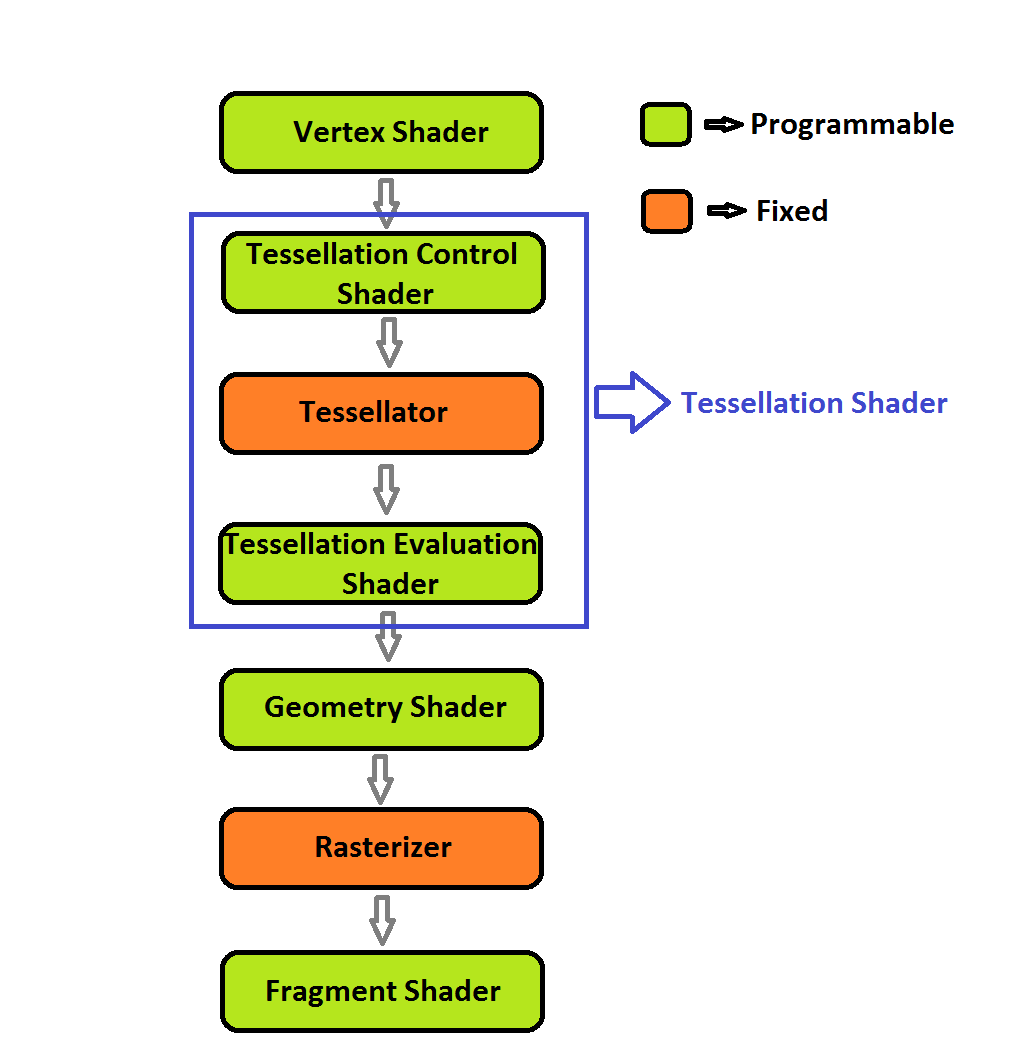
\includegraphics[width=3.5in]{images/OpenGLPipeline.png}
  \caption{Basic OpenGL pipeline}
  \label{fig:openGlPipeline}
\end{figure}

\subsubsection*{Geometry Shader}
All the new vertices and assembled into primitives and passed on to the geometry shader, which then calculated the normal for each face using cross products of the edges. This outputs a single normal per face of the mesh.

\subsubsection*{Fragment Shader}
After determining which pixels are present within a primitive in the Rasterization stage, the pixels are passed into the Fragment shader, where they are colored. I colored the pixels based on the height of the pixel above the ground. I also used the mix function to have a smooth gradient between the colors.

\subsection{Second Render Pass}
For screen space effects like screen space ambient occlusion and depth effects, I created 2 render passes. The first one as mentioned above and the second one with just the Vertex and Fragment shader. This pass just renders 2 triangles to fill up the entire screen. The depth, positions and other information required were pass to this stage from the first one via textures.

\paragraph*{}
\textbf{Screen Space Ambient Occlusion (SSAO)} - This was implemented using a Poisson sphere. The normals were used to calculate how much each pixel is covered by others, to determine the ambient light reaching that point. This was then added to the final rendering. Figure \ref{fig:ambientOcclusion} shows just the ambient occlusion for a generated terrain.

\paragraph*{}
\textbf{Fog} - To give a better scene of depth to the terrain, I added linear fog to the rendering based on distance. The fog becomes thicker as you go further away from the camera. I also added fog in the valleys, which was based on the distance above the ground. This gives an effect of cold mornings in the mountains. Figure \ref{fig:fogDepth} shows the fog based on depth from camera and figure \ref{fig:meshShaded} shows fog based on depth and height.

\subsection{Additional Effects}
In addition to implementing the basic algorithm and the effects using a second render pass, I implemented few other features too.

\subsubsection*{Terrain using heightmaps}
Just a few tweaks to the vertex shader, enabled creating terrain based on heightmaps - Figure \ref{fig:heightmapTerrain}. Heightmaps are grayscale images of elevation data. This data can be used to get the height of vertices on the grid, which then is used to create the terrain. After tessellation, I perturbed the vertices using a noise function to get additional details in the terrain.

\subsubsection*{Terrain Deformation}
I have added an algorithm to deform (blast) parts of terrain approximately based on where you click on the screen. The algorithm shoots a ray into the scene based on the click on the screen and then chooses a random distance after which it creates a blast. It reduces the height of an area around that point based on a random radius value. The blast coordinates are stored as an array and passed into the TES, which flattens the area and then adds some noise, to get an effect of terrain being destroyed. The noise makes sure that the deformed land is not smooth and has some perturbations. Figure \ref{fig:destroy} shows a deformed terrain. The number of deformations is currently limited by the array size passed into the TES as OpenGL 4.0 doesn't support dynamic arrays.

\section{Results}
All the results and images were created by running the algorithm on a NVidia GT650M GPU. It is possible to easily move around the terrain using the keyboard and there are multiple options provided to change the noise parameters while running the application. The frame rate is interactive enough to be able to move around and add/remove fog and other effects without any noticeable lag.

\section{Performance}
Below are few performance numbers based on a grid of 1600 x 2500. These numbers were taken on a NVidia GT650M GPU
\begin{table}[ht]
\begin{center}
\begin{tabular}{|>{\centering\arraybackslash}m{0.5in}|>{\centering\arraybackslash}m{0.5in}
|>{\centering\arraybackslash}m{0.75in}|>{\centering\arraybackslash}m{0.75in}|}
\hline
& Non-Tessellated & Full Tessellation & Camera based Tessellation \\ \hline
Triangle & 160K & 160K*400 & ~20K*400 \\
Mesh & 21 fps & 1.6 fps & 7 fps \\
Shaded & 11 fps & 1.8 fps & 8.5 fps \\
\hline
\end{tabular}
\caption{Performance for a 1024*1024 output image.\newline Inner Tessellation value = 14, Outer Tessellation value = 14}
\label{tb:Perf}
\end{center}
\end{table}
\\
As you can see, the non-tessellated version runs much faster but the terrain lacks all the details. If I tessellate the entire grid, it works at 1.6-1.8 fps. But if I tessellate the terrain based on what the camera can see, the fps increases to 7-8.5 fps. The lesser the tessellation and details you want in the terrain, the better its fps will be. 

\section{Future Work}
There are few things which could be done to make the results better
\begin{itemize}
\item Smoother normals for the terrain - This should give a better look to the generated terrain.
\item Textures for the terrain - It will be good to have textures for different elements in the terrain.
\item Controllable deforming terrain - Deformation position should be totally controllable and maybe should provide the user with a target spot which will be deformed.
\item Separate the terrain into chunks and load chunks only when needed which might improve performance.
\end{itemize}

\section{Conclusion}
For my final project in the GPU Programming class, I created a terrain generator which can create terrain procedurally using noise as well as using heightmaps. The terrain can be tessellated based on user needs and the tessellation can be controlled based on distance from the camera. It has the ability to add ambient occlusion, perform diffuse shading and add fog to the terrain based on distance from camera as well as height above the ground. The application runs at interactive rates where you can easily move around the terrain without any lag.


\section*{Acknowledgements}
I would like to thank Patrick for all the support, feedback and for providing me references as well as Karl, the TA for the course. I would also like to thank my friends and classmates for their feedback.

\bibliographystyle{acmsiggraph}
\bibliography{GPUTerrain}


\begin{figure}[]
  \centering
  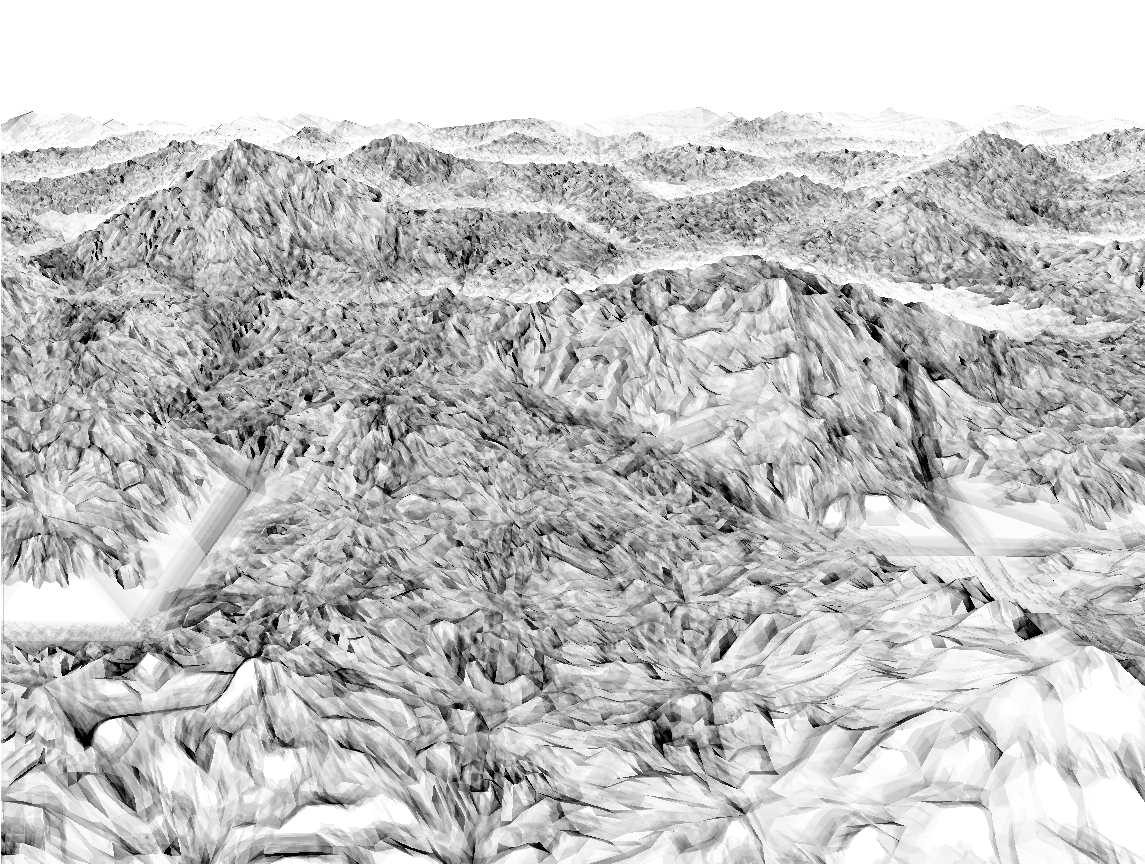
\includegraphics[height=2.5in]{images/AmbientOcclusion.png}
  \caption{Ambient Occlusion}
  \label{fig:ambientOcclusion}
\end{figure}

\begin{figure}[]
  \centering
  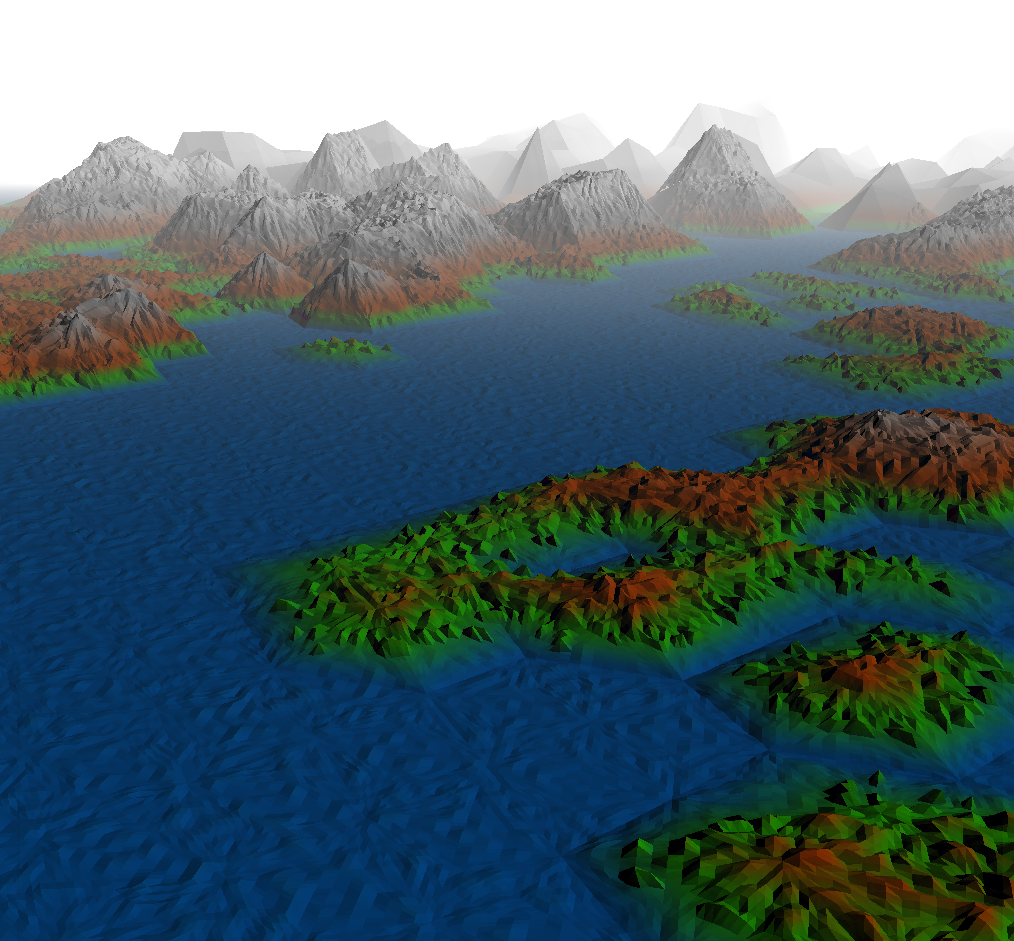
\includegraphics[width=3.1in]{images/NorwayTerrrain1_Heightmap.png}
  \caption{Terrain based on heightmap}
  \label{fig:heightmapTerrain}
\end{figure}

\begin{figure}[]
  \centering
  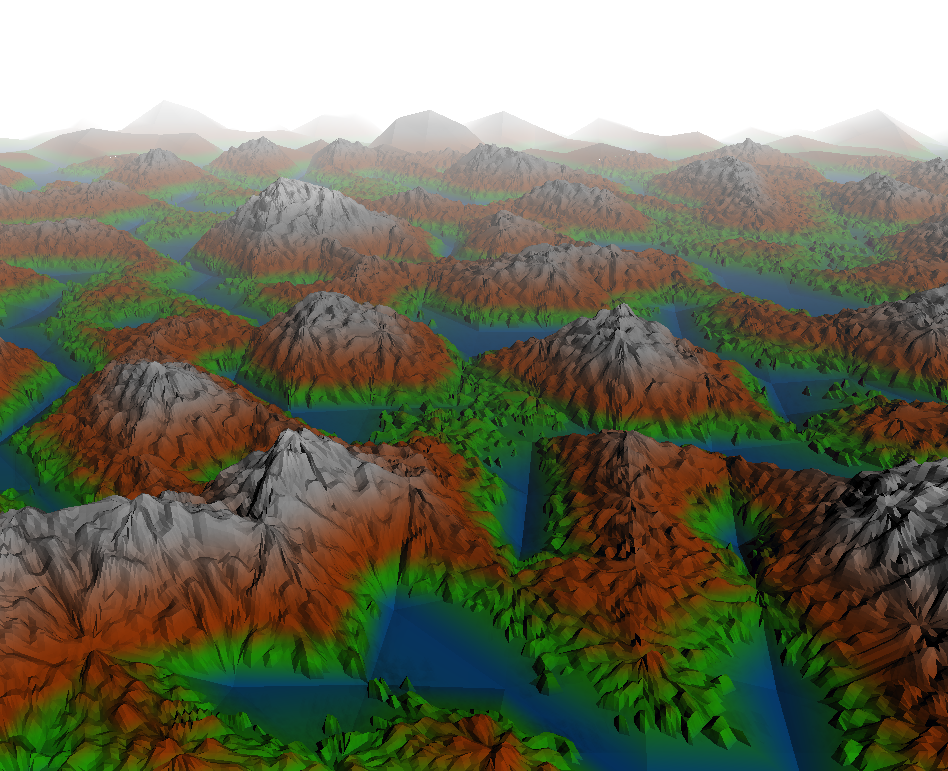
\includegraphics[height=2.45in]{images/Terrain_FogDepth1.png}
  \caption{Fog based on distance from camera}
  \label{fig:fogDepth}
\end{figure}

\begin{figure}[t]
  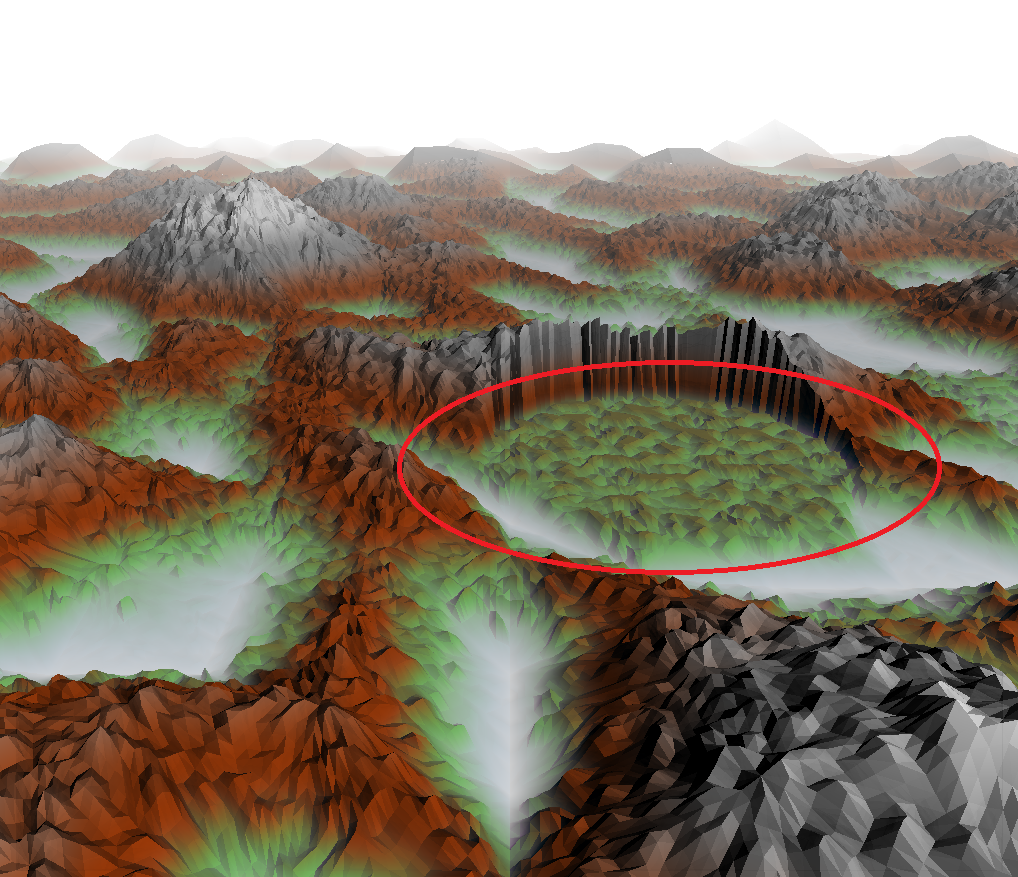
\includegraphics[height=2.5in]{images/Destroy1.png}
  \caption{Destroyed terrain shown by red ellipse}
  \label{fig:destroy}
\end{figure}

\begin{figure}[t]
  
\includegraphics[height=3in]{images/Blank.png}
 % \caption{Destroyed terrain shown by red ellipse}
  %\label{fig:destroy1}
\end{figure}

\begin{figure}[t]
  
\includegraphics[height=3in]{images/Blank.png}
 % \caption{Destroyed terrain shown by red ellipse}
  %\label{fig:destroy1}
\end{figure}

\end{document}
